\section{Collateral feasibility and the timing of funding}
\label{sec:funding}

\subsection{A scalar balance is not a collateral allocation}

CME distinguishes collateral accepted from clearing members from the criteria applicable to account holders through their clearing firms. Public schedules identify eligible assets, haircuts, currency treatment, and concentration limits \citep{CMECollateral,CMEAcceptable}. Assets belonging to different legal accounts cannot be combined merely because a researcher can add their market values.

For a fixed legal account and deadline, let asset $i$ have available amount $c_i$. Allocate $x_{ji}\ge0$ of that asset to requirement $j$. One unit provides credit $a_{ji}\ge0$, where zero means ineligible. Then
\begin{equation}
 \sum_jx_{ji}\le c_i\quad\text{for every asset }i,
 \qquad \sum_i a_{ji}x_{ji}\ge d_j\quad\text{for every requirement }j.
\label{eq:collateral}
\end{equation}
The coefficients contain declared valuation and haircut conversions. Additional concentration or issuer constraints would add rows to this program. The same asset cannot be counted in several requirements without consuming capacity.

\begin{proposition}[Weighted collateral feasibility]\label{prop:collateral}
In the fractional allocation model \eqref{eq:collateral}, with finite assets and requirements, $c_i,d_j,a_{ji}\ge0$, feasibility is equivalent to
\begin{equation}
 \sum_j\lambda_jd_j
 \le\sum_ic_i\max_j\{\lambda_ja_{ji}\}
 \qquad\text{for every }\lambda\in\R_+^J.
\label{eq:collateraldual}
\end{equation}
\end{proposition}
\begin{proof}
For any allocation and nonnegative $\lambda$, weighted supplied credit is at most $\sum_ic_i\max_j\lambda_ja_{ji}$, since each unit of asset $i$ can be assigned only once. This proves necessity.

For sufficiency let $C$ be the compact convex set of credit vectors attainable by allocations satisfying the asset capacities. Requirements are feasible precisely when $d\in C-\R_+^J$. This latter set is closed, convex, and downward closed. If $d$ is outside, a strict separating hyperplane exists. Its normal can be chosen nonnegative: a negative component would give an infinite supremum in that coordinate's downward direction. For its normal $\lambda$, the supremum over $C$ is $\sum_ic_i\max_j\lambda_ja_{ji}$, obtained by assigning each asset to a maximizing requirement. Separation contradicts \eqref{eq:collateraldual}.
\end{proof}

This finite-dimensional result is an application of convex separation and linear-programming duality, not a claim about a complete collateral service. Divisibility, absence of additional caps, and time availability are explicit assumptions. Indivisible assets require an integer model; concentration constraints alter the right-hand support calculation.

\begin{example}[Enough value, too little cash]\label{ex:collateral}
An account has \$5,000 cash and \$20,000 of bond market value. In this synthetic model, bonds receive a 10\% haircut against an initial-margin requirement of \$10,800 but cannot meet the current cash variation payment without a separate sale or financing transaction. Total credited resources are \$23,000.

With a \$4,000 variation payment, allocate \$4,000 cash to variation and \$12,000 bond value to initial margin. This leaves \$1,000 cash and \$8,000 unallocated bonds. With a \$6,000 variation payment, total requirements are only \$16,800, below \$23,000, but the allocation is infeasible because cash is short by \$1,000. In \eqref{eq:collateraldual}, choose weight one on the cash requirement and zero on initial margin to certify the failure.
\end{example}

The haircut is illustrative, not a quoted live CME rate. If bonds can be converted to cash before the deadline, that transaction belongs in the model with its own timing, haircut, cost, and availability. Its existence must not be assumed from the bond's market value alone.

\subsection{Minimum funding is a prefix maximum}

Take an ordered sequence of cash events. Let $r_t\ge0$ be actual receipts available at event $t$ and $d_t\ge0$ obligatory payments, including increases in posted cash collateral where applicable. Releases enter receipts. Assume zero interest, no borrowing after inception, and free retention of receipts. With initial free cash $F$,
\begin{equation}
 b_t=F+\sum_{u=1}^t(r_u-d_u).
\end{equation}

\begin{theorem}[Exact minimum initial funding]\label{thm:funding}
The smallest $F\ge0$ for which every payment can be met in the specified event order is
\begin{equation}
 F^*=\max\left\{0,\max_{1\le t\le T}\sum_{u=1}^t(d_u-r_u)\right\}.
\label{eq:funding}
\end{equation}
\end{theorem}
\begin{proof}
Each constraint $b_t\ge0$ requires $F\ge\sum_{u\le t}(d_u-r_u)$. Their maximum is necessary. Setting $F$ to that maximum satisfies every constraint, establishing sufficiency.
\end{proof}

If a debit precedes a receipt within a nominal clearing cycle, they must be separate events in this theorem. Netting their amounts into one simultaneous event would understate the required funding. The formula measures additional \emph{free cash}; collateral already posted at inception is accounted for separately.

\begin{example}[Identical terminal gain, different liquidity demand]\label{ex:funding}
Hold ten ES contracts from settlement 6,000. Compare settlement paths
\[
 A:(6000,5980,6004),\qquad B:(6000,6002,6004).
\]
Path A produces variation payments $-\$10,000,+\$12,000$; path B produces $+\$1,000,+\$1,000$. Both end with a \$2,000 gain. If initial margin is already posted and unchanged, $F_A^*=\$10,000$ and $F_B^*=0$.

If path A also requires \$5,000 additional cash margin at the first cycle, released at the second, its cumulative free-cash changes become $(-15{,}000,+2{,}000)$. Required initial free cash rises to \$15,000. Starting with \$8,000 leaves a \$7,000 shortfall at the first call despite the positive terminal gain.
\end{example}

\begin{figure}[htbp]
\centering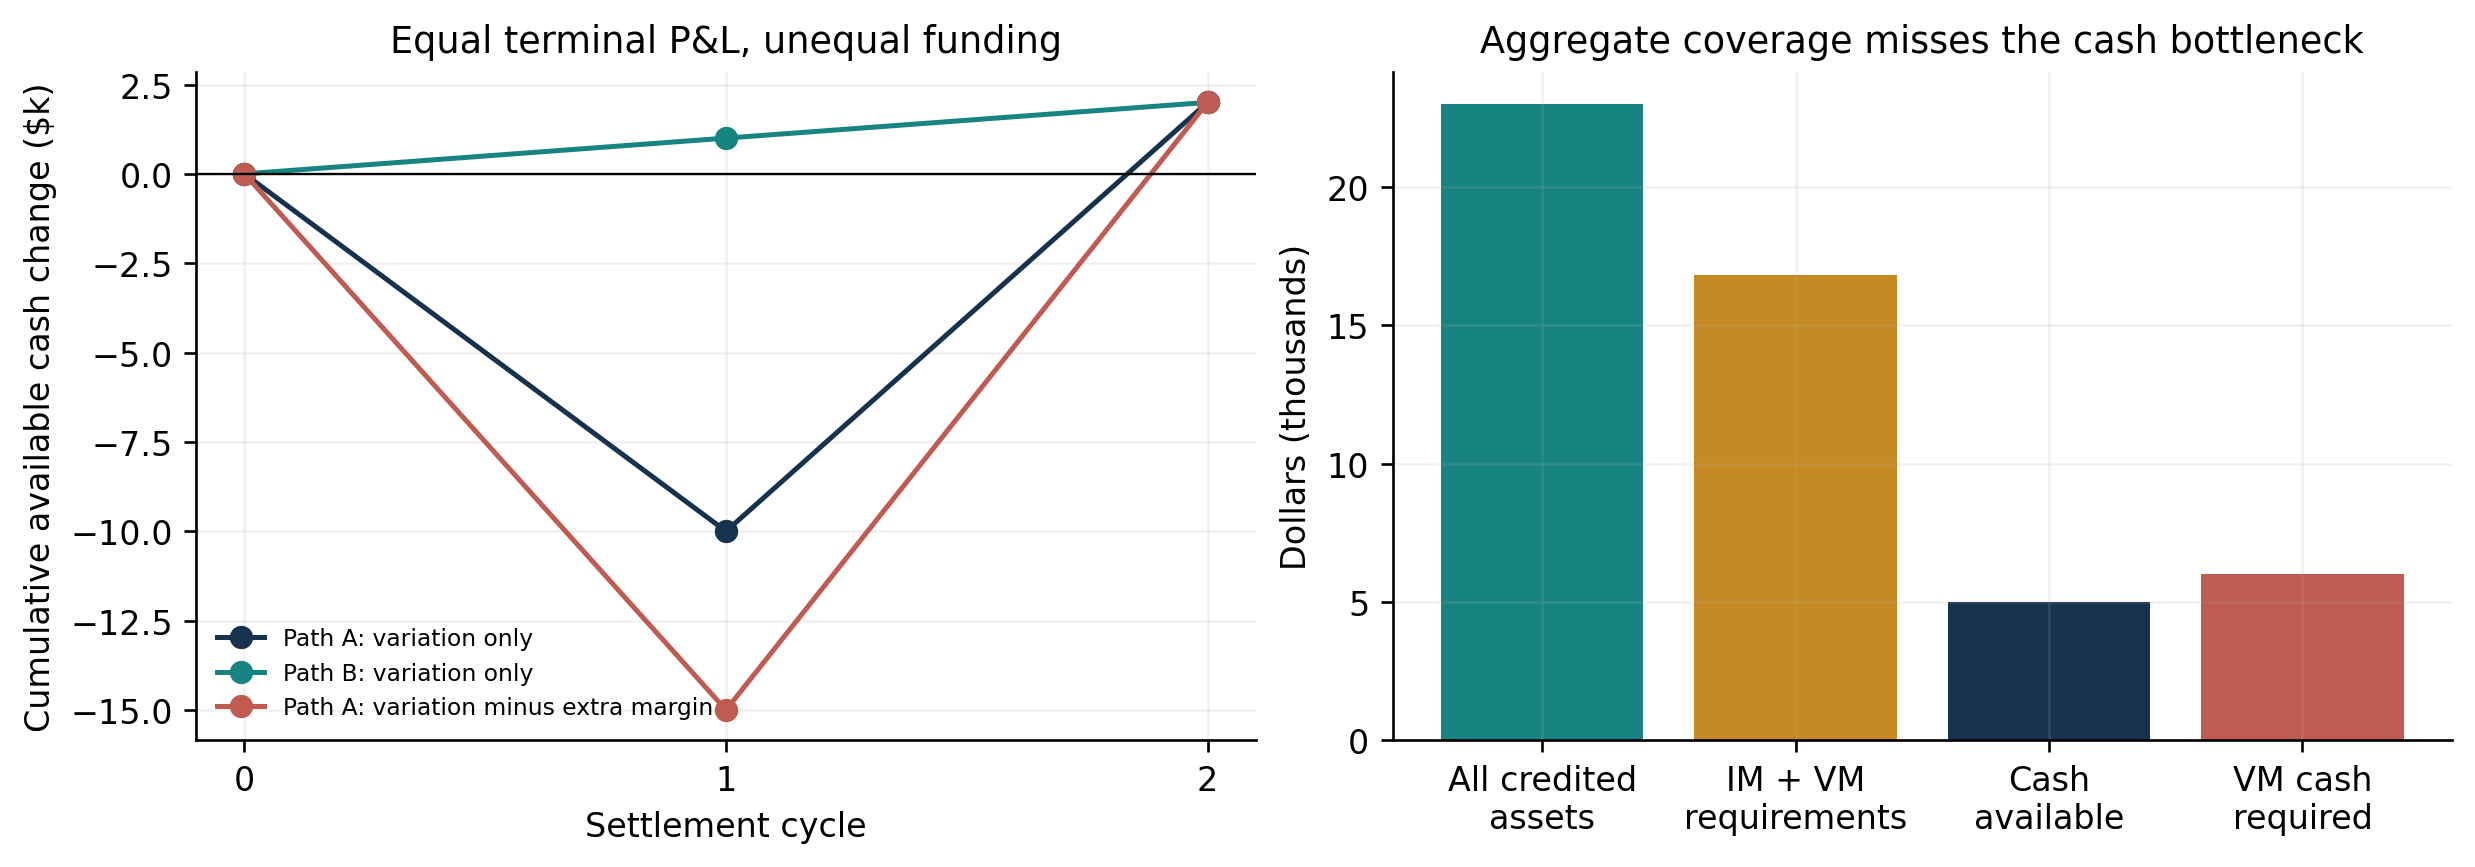
\includegraphics[width=\textwidth]{figures/08_funding.png}
\caption{Two distinct failures of scalar risk summaries. Left: timing changes required funding even with the same final gain. Right: aggregate collateral value cannot replace a cash-eligibility constraint. Parameters are synthetic.}
\label{fig:funding}
\end{figure}

\subsection{Execution under a margin constraint}

Let $u$ be a vector of proposed trades and $z+u$ the resulting positions. A local optimization might trade execution shortfall against a target exposure and a margin charge:
\begin{equation}
 \min_{u\in\mathcal U(X)}
 \left\{\mathrm{IS}(u;X)+\eta M(z+u)
       +\gamma\|z+u-z^{\rm target}\|^2\right\}.
\label{eq:localcontrol}
\end{equation}
The admissible set $\mathcal U(X)$ must enforce integer contracts, available book and recipe capacities, account permissions, price limits, and funding at the relevant deadlines. A favorable marked P\&L is not immediately available cash unless its receipt time is included. A strategy that reduces gross contracts may increase $M$, as Section~\ref{sec:margin} demonstrates.

For a finite-state, finite-action illustration with transition kernel $P_t(x'\mid x,u)$, admissible actions $\mathcal U_t(x)$, and stage cost $c_t$, the continuation value satisfies
\begin{equation}
 J_t(x)=\min_{u\in\mathcal U_t(x)}
 \left[c_t(x,u)+\sum_{x'}P_t(x'\mid x,u)J_{t+1}(x')\right].
\end{equation}
States with no feasible continuation have value $+\infty$. Under partial observation the state for control is a belief such as \eqref{eq:filter}, together with directly known private cash and positions. This equation describes a modeling architecture; no optimal trading policy or empirical transition kernel is estimated here.

The economically relevant feasible set is thus the intersection of execution feasibility, portfolio risk capacity, and deadline-specific funding. Each can bind while the other two appear ample.
\FloatBarrier
